\chapter{High Dynamic Range Imaging}\label{ch:hdr-imaging}

Photographers have long understood that the range of brightness levels in
a real-world scene is considerably larger than the range that can be
captured by a camera's film or imaging sensor.  The luminance of a
outdoor scene can easily span five orders of magnitude, however
typical digital cameras encode the brightness at a single pixel
location using a modest 8-bits (2 orders of magnitude).  Pixels that
fall outside the {\em dynamic range} of the camera sensor will either
be underexposed or overexposed; their values will be at the minimum or
maximum pixel value of the camera, respectively.

Some digital cameras can save RAW images with higher dynamic range
than normal.  These cameras can capture 12 bits per pixel, or 4096
brightness levels.  This expanded dynamic range is often sufficient to
capture scenes with a moderate amount of contrast. To capture scenes
with very high dynamic range you can generate an HDR image from a set
of {\em bracketed} exposures: a group of low dynamic range images of
the exact same scene taken with a set of different exposure settings
that varies from under-exposed to over-exposed.  This technique is
subject of section \ref{sec:hdr_merge}.

The resulting HDR image is generally stored with a channel type of
{\tt float} or {\tt int16} to accomodate the expanded dynamic range.
To store HDR images on disk we recommend using the OpenEXR or TIFF
file formats, both of which support 32-bit floating point channel
types.

Just as capturing HDR images can be challenging, visualizing them is
also difficult.  Print media and most display devices can only manage
about 2 orders of magnitude of dynamic range, whereas an HDR image may
have 5 or more orders of magnitude. Simply scaling the image to the
display range will cause it to look overly dark or washed-out. Section
\ref{sec:tonemapping} discusses a technique called {\em tone mapping}
that reduces the dynamic range of an image while preserving as much as
possible the visual contrasts of the original scene.

\section{Merging Bracketed Exposures}
\label{sec:hdr_merge}

As discussed in the introduction to this chapter, the limited dynamic
range of the sensors on modern cameras necessitates a different
strategy for building true HDR images: exposure backeting.  This frees
us from hardware limitations and allows us to set the dynamic range of
the output image by adjusting the range of exposures in the bracket.
If more dynamic range is needed, one can simply add additional
exposures on either side of the bracket.

\begin{figure}[tbp]
\begin{center}
  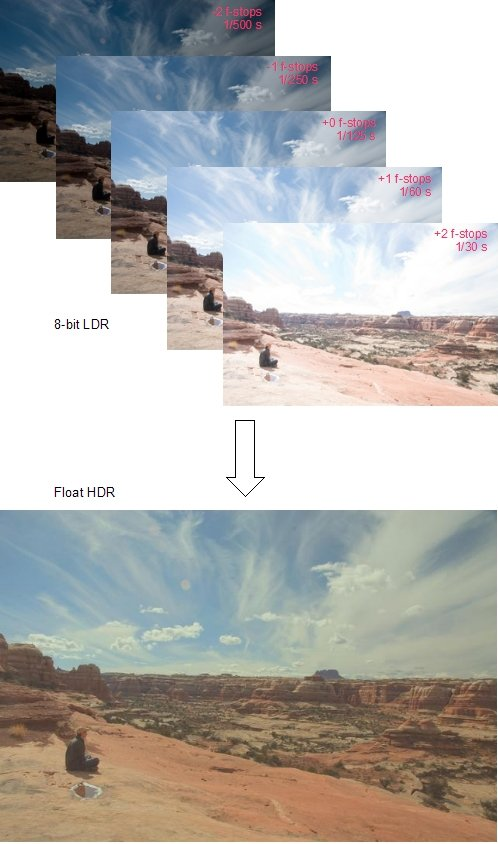
\includegraphics[width=5in]{images/hdr_merge.jpg}
 \end{center}
  \label{fig:hdrmerge}
  \caption{A stack of 8-bit-per-channel LDR images separated by one
    f-stop is merged a floating-point HDR image. The HDR image is
    tone-mapped for display using the Drago operator.}
\end{figure}

For convenience, the exposure ratio between consecutive images is
usually fixed {\em a priori} to guarantee a wide exposure range while
maintaning even brightness overlap between adjacent images in the
bracket. A factor of two is generally recommended.  The shutter speed
is generally the preferred method of varying the exposure in a
bracket; changing the aperture or ISO setting can have the same effect
on exposure but they may change the focus or increase noise.

\subsection{Using HDR Stacks}
The HDR module has a set of free functions that make stitching a stack of LDR
images into an HDR image as simple as one function call. process\_ldr\_images (in 
LDRtoHDR.h) takes a std::vector of ImageViews (with grayscale or RGB pixels
and a floating point channel type), sorted from darkest to brightest. This
function assumes a constant exposure ratio between images; it can be specified
or the default of $\sqrt{2}$ can be used for stacks with a ratio of 1 EV. An
overloaded version also accepts a std::vector$<$vw::Vector$<$double$>$ $>$ by reference,
to return the estimated response curves for each channel.

\begin{verbatim}
/* Generate HDR image from HDR stack. */
typedef ImageView<PixelRGB<double> > Image;
vector<Image> images(num_images);
// ... Read input images ...
// Assume default exposure ratio.
Image hdr_image = process_ldr_images(images);
\end{verbatim}

LDRtoHDRExif.h further defines process\_ldr\_images\_exif, which generates an HDR
image from an array of filenames of LDR images, computing brightness values
from the files' Exif data. Example code usingthis function is in Appendix B. It
also defines another overloaded version of process\_ldr\_images that takes a
std::vector$<$double$>$ of brightness values (as defined by the APEX system \cite{apex})
instead of a constant exposure ratio. These functions do not require the images
to be in any particular order of have a constant exposure ratio.

\subsection{Alignment}
It is crucial for the images in an HDR stack to be aligned, both so
that the resulting HDR image is not blurry and so that the camera
response curve can be estimated accurately.  The best solution is to
take the HDR stack on a tripod, ideally using remote capture.  {\em If
  you are able to take the images on a stationary platform, there is
  no need to perform image alignment in software.}  However, for
handheld photographs, or if dynamic disturbances, such as wind, shake
the camera on the tripod, software alignment is then likely to be
necessary.

For HDR stacks shot with a hand-held camera or otherwise unaligned,
the HDR module includes MTBAlign.h, an implementation of the Mean
Threshold Bitmap (although it actually uses the median) alignment
technique \cite{hdrbook}. MTB alignment thresholds two images on their
respective medians and finds the x- and y-shifts that minimize the
difference of the resulting bitmaps. This technique is well-suited for
HDR stacks as the median threshold bitmap is relatively invariant with
respect to the exposure used to take the photo, whereas edges may fade
in and out. The weakness of MTB alignment is that it only considers
translation. This should be sufficient even for most photos taken
hand-held, but to align images that are rotated or otherwise warped, a
more sophisticated alignment technique should be used (the
InterestPoint module, for example).

\begin{verbatim}
// Find the shift to be applied to img2 to match it most
// closely with img1.

int shift_bits = 6; // Maximum shift of 64 pixels
int shift[2];       // Will hold (x,y) shift

// img1 and img2 assumed to be of type
// ImageView<PixelGray<double> >.
get_exp_shift(img1, img2, shift_bits, shift);
\end{verbatim}

\subsection{Camera Response Curves}
The relation between light entering a camera sensor and the pixel
value that is ultimately recorded is non-linear.  The function that
maps the amount of light on the sensor (the luminance) to the pixel
value is referred to as the camera response curve.  [TODO: Add camera
  response curve figure.]  

\begin{figure}[tbp]
\begin{center}
  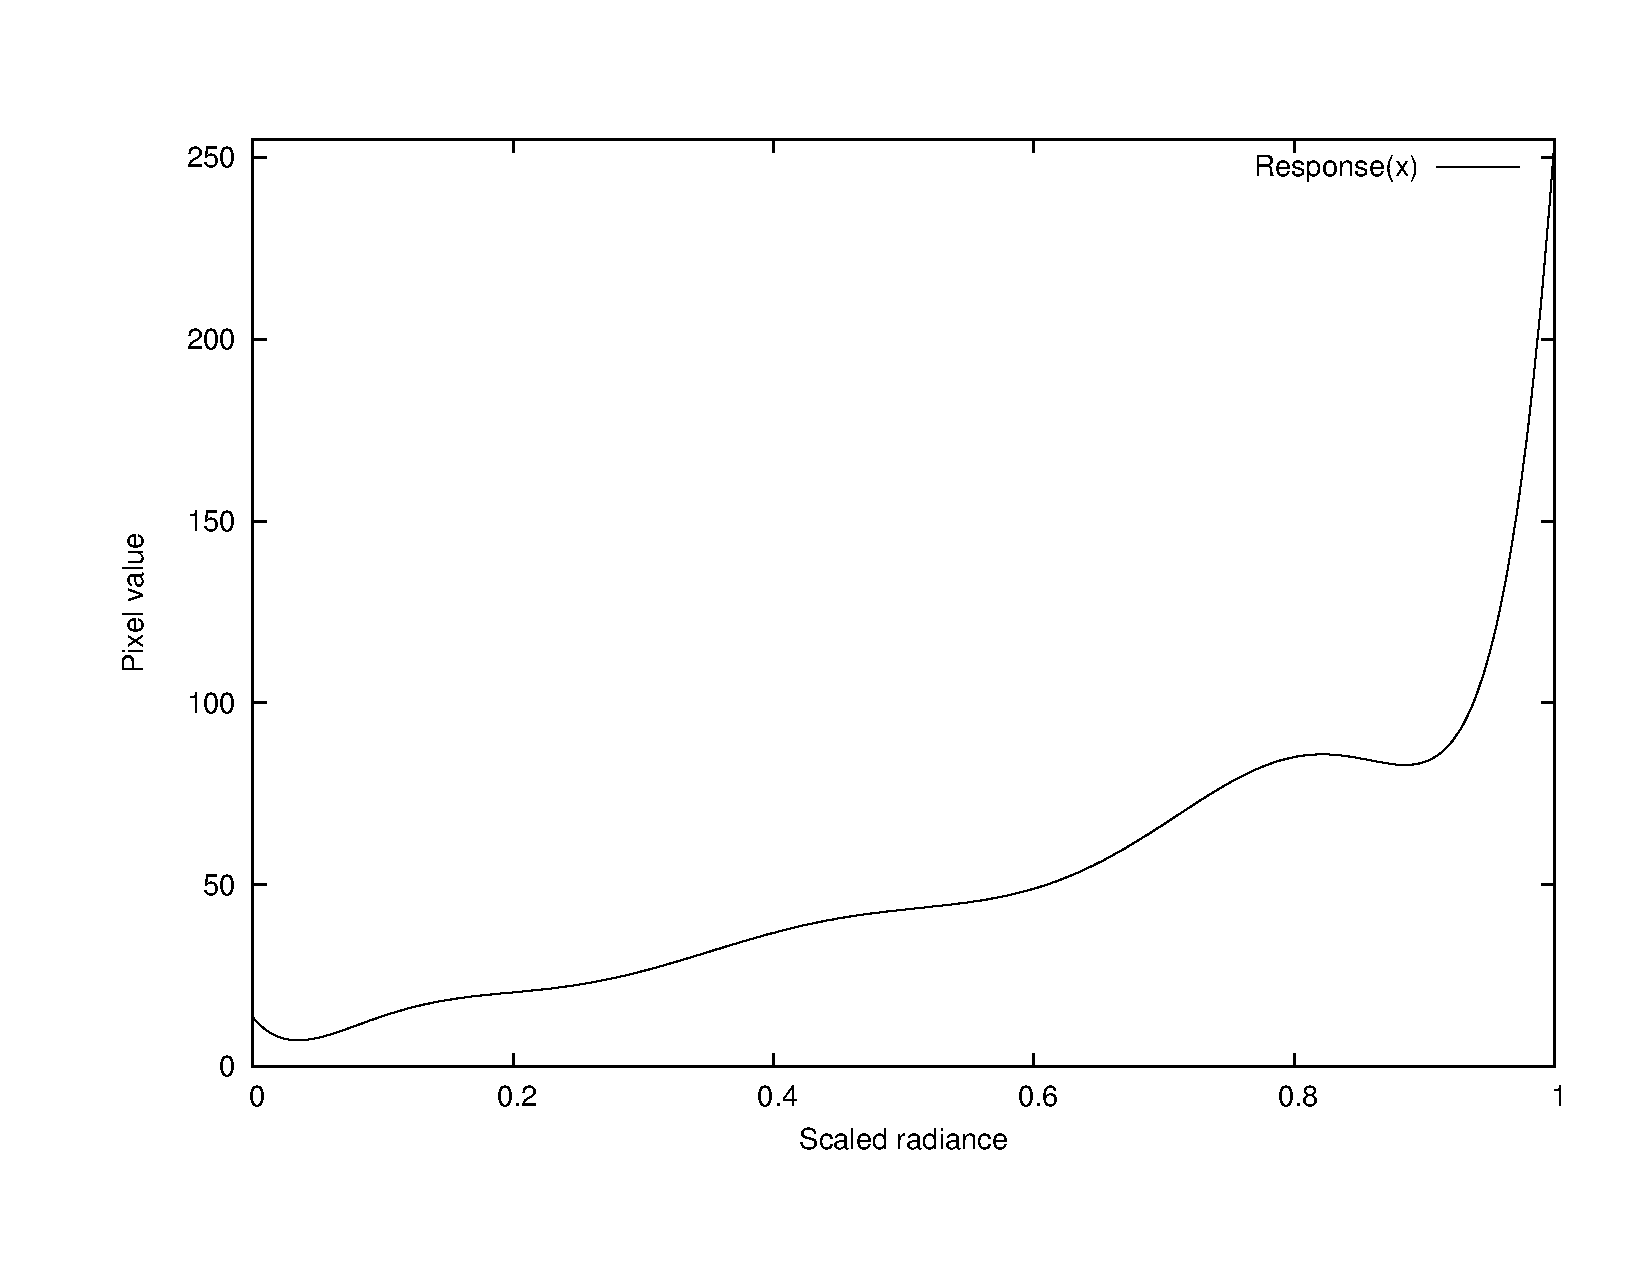
\includegraphics[width=5in]{images/hdr_response.pdf}
 \end{center}
  \label{fig:response}
  \caption{Camera response curve estimated from an HDR stack.}
\end{figure}

To create an HDR image that truly represent the physical brightness
levels in a scene, it is necessary to estimate the inverse of the
camera response curves (we assume a separate curve for each channel)
and apply it to the image data.  That is, we would like to find a
function that, given a pixel value in the image and its exposure
information, returns the luminance of the scene at that point.
CameraCurve.h and CameraCurve.cc implement {\tt
  estimate\_camera\_curve()}, a free function that estimates the
inverse response curve as a polynomial.  This routine takes a matrix
of aligned pixel channel values from an HDR stack and their brightness
ratios. This function is used by LDRtoHDR.h and its relatives; most
users will probably not need to call it directly.

The CameraCurve sources also supply {\tt invert\_curve()}, a free
function that approximates the inverse of a polynomial curve, also as
a polynomial. This is useful to recover the actual camera response
curve (mapping a scaled luminance value to a pixel value) from the
inverse response curve determined by {\t
  estimate\_camera\_curve()}. Re-applying the camera response curve to
an HDR image after tone-mapping can improve the colors and overall
visual appeal. See the code example in Appendix B for an example.

\section{Tone Mapping}
\label{sec:tonemapping}
Since print media and most display technologies are inherently LDR,
an the dynamic range of an HDR image must be compressed before it
can be displayed. Simply scaling the pixel luminances linearly
yields poor results because the human visual system's response to
luminance is approximately logarithmic rather than linear. A linear
scaling tends to lose small details and local contrast, and the
image as a whole will appear under- or over-exposed.

A wide variety of tone-mapping operators have been proposed to
compress the dynamic range of an HDR image while preserving
details and local contrast as much as possible. Using an ideal
tone-mapping operator, the observer of a tone-mapped LDR image
would have a perceptual response matching that of the original
HDR scene. Due to its greater realism, tone-mapping generally
vastly improves the appearance of the displayed image.

There are several broad classes of tone-mapping operators, including
global operators, local operators, and operators that use the
gradient or frequency domains. The HDR module currently includes
one global operator and one local operator; they are described in
the following sections.

\subsection{Global Operators}
Global tone-mapping operators apply the same compressive function to
all pixels in the image. Such operators are implemented in
GlobalToneMap.h/.cc. Currently one such operator is implemented, the
Drago Adaptive Logarithmic Mapping operator.  For algorithm details
see \emph{High Dynamic Range Imaging} \cite{hdrbook} or the original
paper \cite{drago}.  The Drago operator is currently the operator of
choice in the HDR module. It is quite fast, produces good results for
a wide range of images, and can usually be used with its parameters at
default values. Optionally, the parameters bias (controlling contrast,
usually between 0.7 and 0.9), exposure factor (a simple multiplier to
control the overall brightness of the image), and max display
luminance (usually about 100) can be specified.

\begin{verbatim}
/* Apply Drago tone-mapping operator */
ImageView<PixelRGB<float> > tone_mapped = drago_tone_map(hdr_image);
\end{verbatim}

\begin{figure}[tbp]
\begin{center}
  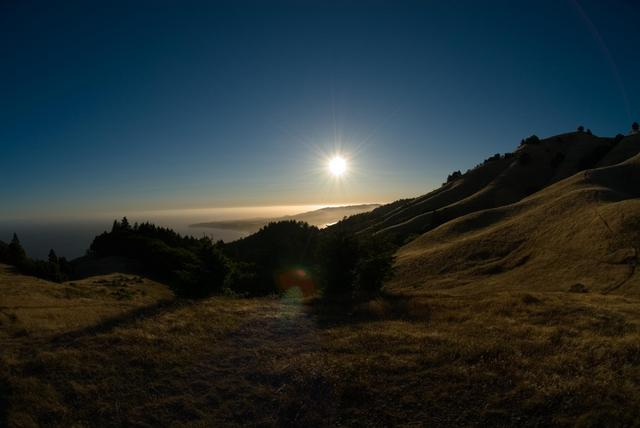
\includegraphics[height=3in]{images/hdr_original.jpg}
  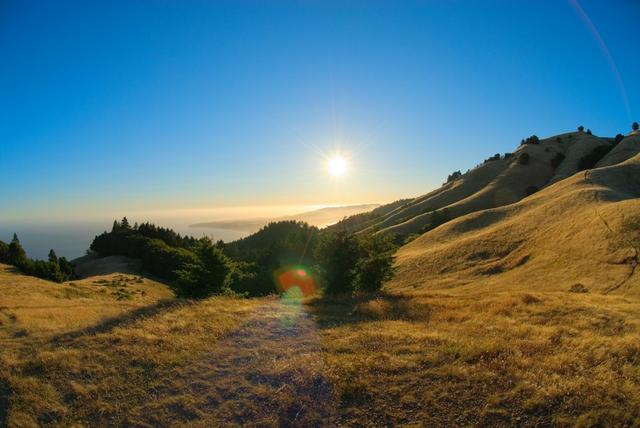
\includegraphics[height=3in]{images/hdr_drago.jpg}
  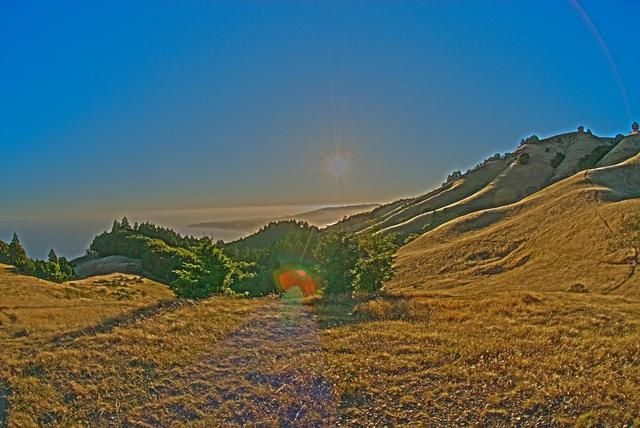
\includegraphics[height=3in]{images/hdr_ashikhmin.jpg}
 \end{center}
  \label{fig:tonemapping}
  \caption{Top: an image taken in 12-bit RAW format. Middle: after
           tone-mapping with the Drago operator. Bottom: after
           tone-mapping with the Ashikhmin operator.}
\end{figure}

\subsection{Local Operators}
Local tone-mapping operators compress a pixel's dynamic range in a way
dependent on the neighborhood of pixels around it. These operators
mimic the local adaptation of the human eye and are capable of more
striking or artistic results than global operators, but they are also
susceptible to artifacts such as excessive haloing and reverse
gradients. LocalToneMap.h/.cc currently implements the Ashikhmin local
tone-mapping operator \cite{ashikhmin}.  It is much slower than the
Drago operator and more prone to artifacts, but may be useful for some
images. Its only parameter is a threshold value (0.5 by default) which
roughly controls the size of the neighborhood used for each pixel. A
threshold value too large will result in haloing.

\begin{verbatim}
/* Apply Ashikhmin tone-mapping operator */
ImageView<PixelRGB<float> > tone_mapped = ashikhmin_tone_map(hdr_image);
\end{verbatim}

\subsection{Using HDR Stacks}
The HDR module has a set of free functions that make stitching a stack of LDR
images into an HDR image as simple as one function call. process\_ldr\_images (in 
LDRtoHDR.h) takes a std::vector of ImageViews (with grayscale or RGB pixels
and a floating point channel type), sorted from darkest to brightest. This
function assumes a constant exposure ratio between images; it can be specified
or the default of $\sqrt{2}$ can be used for stacks with a ratio of 1 EV. An
overloaded version also accepts a std::vector$<$vw::Vector$<$double$>$ $>$ by reference,
to return the estimated response curves for each channel.

\begin{verbatim}
/* Generate HDR image from HDR stack. */
typedef ImageView<PixelRGB<double> > Image;
vector<Image> images(num_images);
// ... Read input images ...
// Assume default exposure ratio.
Image hdr_image = process_ldr_images(images);
\end{verbatim}

LDRtoHDRExif.h further defines process\_ldr\_images\_exif, which generates an HDR
image from an array of filenames of LDR images, computing brightness values
from the files' Exif data. Example code usingthis function is in Appendix B. It
also defines another overloaded version of process\_ldr\_images that takes a
std::vector$<$double$>$ of brightness values (as defined by the APEX system \cite{apex})
instead of a constant exposure ratio. These functions do not require the images
to be in any particular order of have a constant exposure ratio.

\section{Panoramic HDR}
Applying HDR techniques to panoramic images is extremely challenging,
as it is necessary to consider how each individual image is placed in
the full panorama.  LDRtoHDRPano.h contains prototype code for
computing the response curves from a set of panoramic images and
projecting the individual images into the same luminance
space. Blending the resulting images together into a full panorama is
left to a separate blender.

The difficult part is computing the camera response curves from the
panoramic images; it would be simpler to compute and cache the
response curves using a standard HDR stack, but on digital cameras the
response curves may vary with settings. Basically, the areas of the
panorama where two or more individual images overlap are used as HDR
stacks for sampling. The panorama is traversed considering one square
section at a time, so that only those images overlapping that section
need to be loaded (keeping all of the individual images in memory at
once would be too memory-inefficient).  Brightness data is extracted
from the Exif data in the original images.

LDRtoHDRPano.h defines the free function
process\_ldr\_images\_pano. The inputs will likely need to be changed
to accept whatever variety of ImageView(Ref) the panorama alignment
algorithm produces. Currently the inputs are a vector of PanoImage
structs, an optional vector of brightness values for the images
(otherwise Exif is used), the width and height of the full panorama,
and a vector of vw::Vectors to store the computed camera response
curves. PanoImage holds the image's file name, a Rect struct which
holds its dimensions and offset within the panorama, and a
brightness\_multiplier field in which process\_ldr\_images\_pano
stores a multiplier that will project the image into the same
luminance space as the others (after applying the camera curves using
the function psi from LDRtoHDR.h). The outputs are the camera response
curves and the brightness multipliers.

\section{Command Line Utilities}
There are a number of freely available command line utilities which are useful for working
with HDR images. The OpenEXR distribution \cite{openexr} includes several utilities,
including exrdisplay for displaying OpenEXR images. exrtools \cite{exrtools} provides
utilities for converting between OpenEXR and other formats, performing basic operations
on OpenEXR images, and a couple of tone-mapping utilities. pfstools \cite{pfstools} is a
well-integrated set of utilities for reading, writing, manipulating and viewing HDR images.
It has an associated pfstmo project that implements seven of the more prominent tone
mapping operators.

\begin{verbatim}
/* Create a PanoImage struct */
PanoImage img = PanoImage(``img.jpg'', Rect(img_x,
                img_y, width, height), 0);

/* Compute response curves and brightness multipliers */
vector<PanoImage> images;
vector<Vector<double> > curves;
// ... load images ..
process_ldr_images_pano(images, pano_width,
                        pano_height, curves);
\end{verbatim}

\section{List of Files}
\begin{description}
\item[CameraCurve.h, cc] Functions for estimating camera response curves and inverting curves.
\item[ExifData.h, cc] Class for reading Exif data from JPEG or TIFF images. Offers access to
any tag referenced by tag ID.
\item[ExifView.h, cc] Class providing a convenient interface for extracting exposure data
from Exif.
\item[GlobalToneMap.h, cc] Functions for applying global tone-mapping operators. Currently
implements the Drago operator.
\item[GradientDomain.h, cc] Functions for applying gradient domain tone-mapping operator.
Currently implements the Fattal operator.
\item[LDRtoHDR.h] Functions for generating an HDR image from an HDR stack of LDR images
using either a constant exposure ratio.
\item[LDRtoHDRExif.h] Extends functionality of LDRtoHDR.h to use exposure data from Exif.
\item[LDRtoHDRPano.h] Estimates response curves and brightness multipliers for aligned
images in a panorama.
\item[LocalToneMap.h, cc] Functions for applying local tone-mapping operators. Currently
implements the Ashikhmin operator.
\item[print\_exif.cc] An example program which uses ExifView to display some Exif data.
\end{description}

\section{Full Code Example}
\begin{verbatim}
/* ExifHDR_test.cc
 * 
 * This is a simple test program that stitches an
 * Exif-tagged HDR stack into an HDR image,
 * performs tone-mapping, and saves several
 * versions with different post-processing applied
 * for comparison. Usually the best image is
 * produced by re-applying the camera response
 * curves and then gamma correcting.
 */

#include <vw/Image/ImageView.h>
#include <vw/FileIO.h>
#include <vw/Image/Algorithms.h>
#include <vw/Image/ImageMath.h>
#include <vw/HDR/LDRtoHDRExif.h>
#include <vw/HDR/GlobalToneMap.h>

#include <stdio.h>
#include <vector>

using namespace std;
using namespace vw;
using namespace vw::HDR;

int main(int argc, char** argv) {
  typedef ImageView<PixelRGB<double> > Image;

  vector<Vector<double> > curves;
  vector<string> files;
  for(int i = 1; i < argc; i++)
    files.push_back(argv[i]);
  // Process HDR stack using Exif tags
  Image hdr_exif = process_ldr_images_exif(files,
                                          curves);
  write_image("hdr.exr", hdr_exif);

  // Apply Drago tone-mapping operator.
  Image tone_mapped = drago_tone_map(hdr_exif);
  write_image("tm.jpg", tone_mapped);

  // Apply gamma correction and save.
  Image gamma = pow(tone_mapped, 1.0/2.2);
  write_image("tm_gamma.jpg", gamma);

  // Re-apply camera response curves and save.
  // First must invert curves calculated earlier.
  vector<Vector<double> > inverse_curves(curves.size());
  for (int i = 0; i < curves.size(); i++) {
    invert_curve(curves[i], inverse_curves[i],
                 VW_HDR_RESPONSE_POLYNOMIAL_ORDER);
  }
  psi(tone_mapped, inverse_curves);
  write_image("tm_curved.jpg", tone_mapped);

  // Apply gamma correction after response curves.
  // Usually gives best results.
  Image tm_c_g = pow(tone_mapped, 1.0/2.2);
  write_image("tm_c_g.jpg", tm_c_g);  

  return 0;
}
\end{verbatim}

\begin{thebibliography}{1}

\bibitem{ashikhmin} Ashikhmin, Michael, ``A Tone Mapping Algorithm for High Contrast Images,''
{\em Eurographics Workshop on Rendering}, 2002: 1--11.

\bibitem{exrtools} Biggs, Billy, ``exrtools: a collection of utilities for manipulating
OpenEXR images,'', 2004, http://scanline.ca/exrtools/.

\bibitem{drago} Drago et al., ``Adaptive Logarithmic Mapping For Displaying High Contrast Scenes,''
{\em Eurographics}, {\bf 22}(3), 2003.

\bibitem{exif} ``Exchangeable image file format for digital still cameras: Exif Version 2.2'',
(Japan Electronics and Information Technology Industries Assocation, 2002),
http://www.exif.org/specifications.html.

\bibitem{fattal} Fattal, Raanan, et. al, ``Gradient Domain High Dynamic Range Compression,''
{\em ACM Transactions on Graphics}, 2002.

\bibitem{openexr} Industrial Light and Magic, ``OpenEXR,'' (Lucasfilm Ltd., 2006),
http://www.openexr.com.

\bibitem{apex} Kerr, Douglas, ``APEX--The Additive System of Photographic Exposure,'' 2006,
http://doug.kerr.home.att.net/pumpkin/APEX.pdf.

\bibitem{pfstools} Mantiuk, Rafal, and Grzegorz Krawczyk, ``pfstools for HDR processing,'' 2006,
http://www.mpi-inf.mpg.de/resources/pfstools/.

\bibitem{reinhard} Reinhard, Erik, et. al. ``Photographic Tone Reproduction for Digital Images,''
{\em ACM Transactions on Graphics}, 2002.

\bibitem{hdrbook} Reinhard, Erik, Greg Ward, Sumanta Pattanaik, and Paul Debevec,
{\em High Dynamic Range Imaging}, (Boston: Elsevier, 2006).

\bibitem{jhead} Wandel, Matthias, ``Exif Jpeg header and thumbnail manipulator program,'' 2006,
http://www.sentex.net/~mwandel/jhead/.

\bibitem{ward} Ward, Greg, et al., ``A Visibility Matching Tone Reproduction Operator for High Dynamic Range Scenes,''
{\em IEEE Transactions on Visualization and Computer Graphics}, 1997.

\end{thebibliography}
